% Created by tikzDevice version 0.12.3.1 on 2022-08-31 08:50:14
% !TEX encoding = UTF-8 Unicode
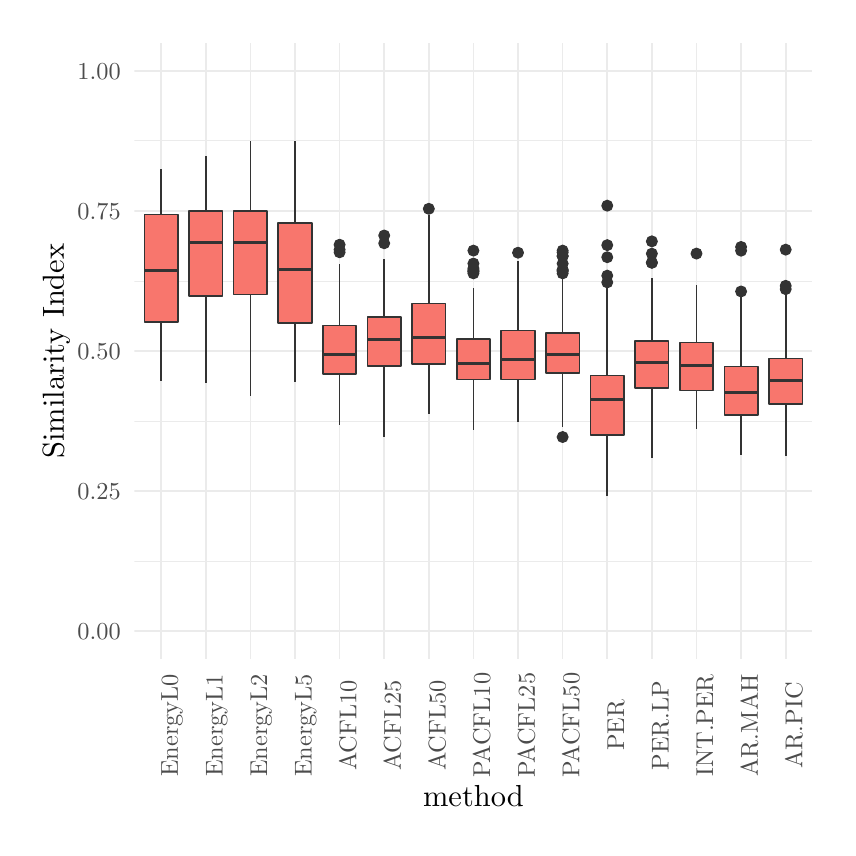
\begin{tikzpicture}[x=1pt,y=1pt]
\definecolor{fillColor}{RGB}{255,255,255}
\path[use as bounding box,fill=fillColor,fill opacity=0.00] (0,0) rectangle (289.08,289.08);
\begin{scope}
\path[clip] ( 38.56, 60.92) rectangle (283.58,283.58);
\definecolor{drawColor}{gray}{0.92}

\path[draw=drawColor,line width= 0.3pt,line join=round] ( 38.56, 96.34) --
	(283.58, 96.34);

\path[draw=drawColor,line width= 0.3pt,line join=round] ( 38.56,146.95) --
	(283.58,146.95);

\path[draw=drawColor,line width= 0.3pt,line join=round] ( 38.56,197.55) --
	(283.58,197.55);

\path[draw=drawColor,line width= 0.3pt,line join=round] ( 38.56,248.16) --
	(283.58,248.16);

\path[draw=drawColor,line width= 0.6pt,line join=round] ( 38.56, 71.04) --
	(283.58, 71.04);

\path[draw=drawColor,line width= 0.6pt,line join=round] ( 38.56,121.64) --
	(283.58,121.64);

\path[draw=drawColor,line width= 0.6pt,line join=round] ( 38.56,172.25) --
	(283.58,172.25);

\path[draw=drawColor,line width= 0.6pt,line join=round] ( 38.56,222.85) --
	(283.58,222.85);

\path[draw=drawColor,line width= 0.6pt,line join=round] ( 38.56,273.46) --
	(283.58,273.46);

\path[draw=drawColor,line width= 0.6pt,line join=round] ( 48.23, 60.92) --
	( 48.23,283.58);

\path[draw=drawColor,line width= 0.6pt,line join=round] ( 64.35, 60.92) --
	( 64.35,283.58);

\path[draw=drawColor,line width= 0.6pt,line join=round] ( 80.47, 60.92) --
	( 80.47,283.58);

\path[draw=drawColor,line width= 0.6pt,line join=round] ( 96.59, 60.92) --
	( 96.59,283.58);

\path[draw=drawColor,line width= 0.6pt,line join=round] (112.71, 60.92) --
	(112.71,283.58);

\path[draw=drawColor,line width= 0.6pt,line join=round] (128.83, 60.92) --
	(128.83,283.58);

\path[draw=drawColor,line width= 0.6pt,line join=round] (144.95, 60.92) --
	(144.95,283.58);

\path[draw=drawColor,line width= 0.6pt,line join=round] (161.07, 60.92) --
	(161.07,283.58);

\path[draw=drawColor,line width= 0.6pt,line join=round] (177.19, 60.92) --
	(177.19,283.58);

\path[draw=drawColor,line width= 0.6pt,line join=round] (193.31, 60.92) --
	(193.31,283.58);

\path[draw=drawColor,line width= 0.6pt,line join=round] (209.43, 60.92) --
	(209.43,283.58);

\path[draw=drawColor,line width= 0.6pt,line join=round] (225.55, 60.92) --
	(225.55,283.58);

\path[draw=drawColor,line width= 0.6pt,line join=round] (241.67, 60.92) --
	(241.67,283.58);

\path[draw=drawColor,line width= 0.6pt,line join=round] (257.79, 60.92) --
	(257.79,283.58);

\path[draw=drawColor,line width= 0.6pt,line join=round] (273.91, 60.92) --
	(273.91,283.58);
\definecolor{drawColor}{gray}{0.20}

\path[draw=drawColor,line width= 0.6pt,line join=round] ( 48.23,221.62) -- ( 48.23,237.95);

\path[draw=drawColor,line width= 0.6pt,line join=round] ( 48.23,182.79) -- ( 48.23,161.29);
\definecolor{fillColor}{RGB}{248,118,109}

\path[draw=drawColor,line width= 0.6pt,line join=round,line cap=round,fill=fillColor] ( 42.18,221.62) --
	( 42.18,182.79) --
	( 54.27,182.79) --
	( 54.27,221.62) --
	( 42.18,221.62) --
	cycle;

\path[draw=drawColor,line width= 1.1pt,line join=round] ( 42.18,201.28) -- ( 54.27,201.28);

\path[draw=drawColor,line width= 0.6pt,line join=round] ( 64.35,222.85) -- ( 64.35,242.79);

\path[draw=drawColor,line width= 0.6pt,line join=round] ( 64.35,192.11) -- ( 64.35,160.82);

\path[draw=drawColor,line width= 0.6pt,line join=round,line cap=round,fill=fillColor] ( 58.30,222.85) --
	( 58.30,192.11) --
	( 70.39,192.11) --
	( 70.39,222.85) --
	( 58.30,222.85) --
	cycle;

\path[draw=drawColor,line width= 1.1pt,line join=round] ( 58.30,211.49) -- ( 70.39,211.49);

\path[draw=drawColor,line width= 0.6pt,line join=round] ( 80.47,222.73) -- ( 80.47,248.09);

\path[draw=drawColor,line width= 0.6pt,line join=round] ( 80.47,192.62) -- ( 80.47,156.15);

\path[draw=drawColor,line width= 0.6pt,line join=round,line cap=round,fill=fillColor] ( 74.42,222.73) --
	( 74.42,192.62) --
	( 86.51,192.62) --
	( 86.51,222.73) --
	( 74.42,222.73) --
	cycle;

\path[draw=drawColor,line width= 1.1pt,line join=round] ( 74.42,211.48) -- ( 86.51,211.48);

\path[draw=drawColor,line width= 0.6pt,line join=round] ( 96.59,218.57) -- ( 96.59,248.09);

\path[draw=drawColor,line width= 0.6pt,line join=round] ( 96.59,182.38) -- ( 96.59,161.00);

\path[draw=drawColor,line width= 0.6pt,line join=round,line cap=round,fill=fillColor] ( 90.54,218.57) --
	( 90.54,182.38) --
	(102.63,182.38) --
	(102.63,218.57) --
	( 90.54,218.57) --
	cycle;

\path[draw=drawColor,line width= 1.1pt,line join=round] ( 90.54,201.60) -- (102.63,201.60);
\definecolor{fillColor}{gray}{0.20}

\path[draw=drawColor,line width= 0.4pt,line join=round,line cap=round,fill=fillColor] (112.71,208.86) circle (  1.96);

\path[draw=drawColor,line width= 0.4pt,line join=round,line cap=round,fill=fillColor] (112.71,207.91) circle (  1.96);

\path[draw=drawColor,line width= 0.4pt,line join=round,line cap=round,fill=fillColor] (112.71,210.65) circle (  1.96);

\path[draw=drawColor,line width= 0.6pt,line join=round] (112.71,181.41) -- (112.71,203.51);

\path[draw=drawColor,line width= 0.6pt,line join=round] (112.71,164.03) -- (112.71,145.66);
\definecolor{fillColor}{RGB}{248,118,109}

\path[draw=drawColor,line width= 0.6pt,line join=round,line cap=round,fill=fillColor] (106.66,181.41) --
	(106.66,164.03) --
	(118.75,164.03) --
	(118.75,181.41) --
	(106.66,181.41) --
	cycle;

\path[draw=drawColor,line width= 1.1pt,line join=round] (106.66,171.13) -- (118.75,171.13);
\definecolor{fillColor}{gray}{0.20}

\path[draw=drawColor,line width= 0.4pt,line join=round,line cap=round,fill=fillColor] (128.83,213.98) circle (  1.96);

\path[draw=drawColor,line width= 0.4pt,line join=round,line cap=round,fill=fillColor] (128.83,211.17) circle (  1.96);

\path[draw=drawColor,line width= 0.6pt,line join=round] (128.83,184.46) -- (128.83,205.31);

\path[draw=drawColor,line width= 0.6pt,line join=round] (128.83,166.85) -- (128.83,141.19);
\definecolor{fillColor}{RGB}{248,118,109}

\path[draw=drawColor,line width= 0.6pt,line join=round,line cap=round,fill=fillColor] (122.78,184.46) --
	(122.78,166.85) --
	(134.87,166.85) --
	(134.87,184.46) --
	(122.78,184.46) --
	cycle;

\path[draw=drawColor,line width= 1.1pt,line join=round] (122.78,176.43) -- (134.87,176.43);
\definecolor{fillColor}{gray}{0.20}

\path[draw=drawColor,line width= 0.4pt,line join=round,line cap=round,fill=fillColor] (144.95,223.63) circle (  1.96);

\path[draw=drawColor,line width= 0.6pt,line join=round] (144.95,189.39) -- (144.95,221.50);

\path[draw=drawColor,line width= 0.6pt,line join=round] (144.95,167.61) -- (144.95,149.45);
\definecolor{fillColor}{RGB}{248,118,109}

\path[draw=drawColor,line width= 0.6pt,line join=round,line cap=round,fill=fillColor] (138.90,189.39) --
	(138.90,167.61) --
	(150.99,167.61) --
	(150.99,189.39) --
	(138.90,189.39) --
	cycle;

\path[draw=drawColor,line width= 1.1pt,line join=round] (138.90,177.20) -- (150.99,177.20);
\definecolor{fillColor}{gray}{0.20}

\path[draw=drawColor,line width= 0.4pt,line join=round,line cap=round,fill=fillColor] (161.07,201.08) circle (  1.96);

\path[draw=drawColor,line width= 0.4pt,line join=round,line cap=round,fill=fillColor] (161.07,201.57) circle (  1.96);

\path[draw=drawColor,line width= 0.4pt,line join=round,line cap=round,fill=fillColor] (161.07,208.52) circle (  1.96);

\path[draw=drawColor,line width= 0.4pt,line join=round,line cap=round,fill=fillColor] (161.07,203.84) circle (  1.96);

\path[draw=drawColor,line width= 0.4pt,line join=round,line cap=round,fill=fillColor] (161.07,200.30) circle (  1.96);

\path[draw=drawColor,line width= 0.4pt,line join=round,line cap=round,fill=fillColor] (161.07,202.14) circle (  1.96);

\path[draw=drawColor,line width= 0.4pt,line join=round,line cap=round,fill=fillColor] (161.07,200.94) circle (  1.96);

\path[draw=drawColor,line width= 0.6pt,line join=round] (161.07,176.51) -- (161.07,195.08);

\path[draw=drawColor,line width= 0.6pt,line join=round] (161.07,161.97) -- (161.07,143.80);
\definecolor{fillColor}{RGB}{248,118,109}

\path[draw=drawColor,line width= 0.6pt,line join=round,line cap=round,fill=fillColor] (155.02,176.51) --
	(155.02,161.97) --
	(167.11,161.97) --
	(167.11,176.51) --
	(155.02,176.51) --
	cycle;

\path[draw=drawColor,line width= 1.1pt,line join=round] (155.02,167.82) -- (167.11,167.82);
\definecolor{fillColor}{gray}{0.20}

\path[draw=drawColor,line width= 0.4pt,line join=round,line cap=round,fill=fillColor] (177.19,207.76) circle (  1.96);

\path[draw=drawColor,line width= 0.6pt,line join=round] (177.19,179.60) -- (177.19,204.90);

\path[draw=drawColor,line width= 0.6pt,line join=round] (177.19,161.96) -- (177.19,146.70);
\definecolor{fillColor}{RGB}{248,118,109}

\path[draw=drawColor,line width= 0.6pt,line join=round,line cap=round,fill=fillColor] (171.14,179.60) --
	(171.14,161.96) --
	(183.23,161.96) --
	(183.23,179.60) --
	(171.14,179.60) --
	cycle;

\path[draw=drawColor,line width= 1.1pt,line join=round] (171.14,169.26) -- (183.23,169.26);
\definecolor{fillColor}{gray}{0.20}

\path[draw=drawColor,line width= 0.4pt,line join=round,line cap=round,fill=fillColor] (193.31,203.82) circle (  1.96);

\path[draw=drawColor,line width= 0.4pt,line join=round,line cap=round,fill=fillColor] (193.31,201.20) circle (  1.96);

\path[draw=drawColor,line width= 0.4pt,line join=round,line cap=round,fill=fillColor] (193.31,201.71) circle (  1.96);

\path[draw=drawColor,line width= 0.4pt,line join=round,line cap=round,fill=fillColor] (193.31,208.52) circle (  1.96);

\path[draw=drawColor,line width= 0.4pt,line join=round,line cap=round,fill=fillColor] (193.31,206.53) circle (  1.96);

\path[draw=drawColor,line width= 0.4pt,line join=round,line cap=round,fill=fillColor] (193.31,200.30) circle (  1.96);

\path[draw=drawColor,line width= 0.4pt,line join=round,line cap=round,fill=fillColor] (193.31,141.16) circle (  1.96);

\path[draw=drawColor,line width= 0.4pt,line join=round,line cap=round,fill=fillColor] (193.31,206.53) circle (  1.96);

\path[draw=drawColor,line width= 0.4pt,line join=round,line cap=round,fill=fillColor] (193.31,207.82) circle (  1.96);

\path[draw=drawColor,line width= 0.4pt,line join=round,line cap=round,fill=fillColor] (193.31,201.19) circle (  1.96);

\path[draw=drawColor,line width= 0.6pt,line join=round] (193.31,178.71) -- (193.31,199.00);

\path[draw=drawColor,line width= 0.6pt,line join=round] (193.31,164.34) -- (193.31,144.69);
\definecolor{fillColor}{RGB}{248,118,109}

\path[draw=drawColor,line width= 0.6pt,line join=round,line cap=round,fill=fillColor] (187.26,178.71) --
	(187.26,164.34) --
	(199.35,164.34) --
	(199.35,178.71) --
	(187.26,178.71) --
	cycle;

\path[draw=drawColor,line width= 1.1pt,line join=round] (187.26,170.89) -- (199.35,170.89);
\definecolor{fillColor}{gray}{0.20}

\path[draw=drawColor,line width= 0.4pt,line join=round,line cap=round,fill=fillColor] (209.43,197.05) circle (  1.96);

\path[draw=drawColor,line width= 0.4pt,line join=round,line cap=round,fill=fillColor] (209.43,206.13) circle (  1.96);

\path[draw=drawColor,line width= 0.4pt,line join=round,line cap=round,fill=fillColor] (209.43,210.49) circle (  1.96);

\path[draw=drawColor,line width= 0.4pt,line join=round,line cap=round,fill=fillColor] (209.43,199.47) circle (  1.96);

\path[draw=drawColor,line width= 0.4pt,line join=round,line cap=round,fill=fillColor] (209.43,224.76) circle (  1.96);

\path[draw=drawColor,line width= 0.6pt,line join=round] (209.43,163.33) -- (209.43,195.51);

\path[draw=drawColor,line width= 0.6pt,line join=round] (209.43,141.82) -- (209.43,119.88);
\definecolor{fillColor}{RGB}{248,118,109}

\path[draw=drawColor,line width= 0.6pt,line join=round,line cap=round,fill=fillColor] (203.38,163.33) --
	(203.38,141.82) --
	(215.47,141.82) --
	(215.47,163.33) --
	(203.38,163.33) --
	cycle;

\path[draw=drawColor,line width= 1.1pt,line join=round] (203.38,154.87) -- (215.47,154.87);
\definecolor{fillColor}{gray}{0.20}

\path[draw=drawColor,line width= 0.4pt,line join=round,line cap=round,fill=fillColor] (225.55,207.42) circle (  1.96);

\path[draw=drawColor,line width= 0.4pt,line join=round,line cap=round,fill=fillColor] (225.55,211.86) circle (  1.96);

\path[draw=drawColor,line width= 0.4pt,line join=round,line cap=round,fill=fillColor] (225.55,204.13) circle (  1.96);

\path[draw=drawColor,line width= 0.4pt,line join=round,line cap=round,fill=fillColor] (225.55,204.17) circle (  1.96);

\path[draw=drawColor,line width= 0.6pt,line join=round] (225.55,175.80) -- (225.55,198.54);

\path[draw=drawColor,line width= 0.6pt,line join=round] (225.55,158.76) -- (225.55,133.63);
\definecolor{fillColor}{RGB}{248,118,109}

\path[draw=drawColor,line width= 0.6pt,line join=round,line cap=round,fill=fillColor] (219.50,175.80) --
	(219.50,158.76) --
	(231.59,158.76) --
	(231.59,175.80) --
	(219.50,175.80) --
	cycle;

\path[draw=drawColor,line width= 1.1pt,line join=round] (219.50,168.07) -- (231.59,168.07);
\definecolor{fillColor}{gray}{0.20}

\path[draw=drawColor,line width= 0.4pt,line join=round,line cap=round,fill=fillColor] (241.67,207.45) circle (  1.96);

\path[draw=drawColor,line width= 0.6pt,line join=round] (241.67,175.26) -- (241.67,196.23);

\path[draw=drawColor,line width= 0.6pt,line join=round] (241.67,158.02) -- (241.67,143.99);
\definecolor{fillColor}{RGB}{248,118,109}

\path[draw=drawColor,line width= 0.6pt,line join=round,line cap=round,fill=fillColor] (235.62,175.26) --
	(235.62,158.02) --
	(247.71,158.02) --
	(247.71,175.26) --
	(235.62,175.26) --
	cycle;

\path[draw=drawColor,line width= 1.1pt,line join=round] (235.62,166.87) -- (247.71,166.87);
\definecolor{fillColor}{gray}{0.20}

\path[draw=drawColor,line width= 0.4pt,line join=round,line cap=round,fill=fillColor] (257.79,193.76) circle (  1.96);

\path[draw=drawColor,line width= 0.4pt,line join=round,line cap=round,fill=fillColor] (257.79,209.84) circle (  1.96);

\path[draw=drawColor,line width= 0.4pt,line join=round,line cap=round,fill=fillColor] (257.79,208.49) circle (  1.96);

\path[draw=drawColor,line width= 0.6pt,line join=round] (257.79,166.63) -- (257.79,192.64);

\path[draw=drawColor,line width= 0.6pt,line join=round] (257.79,149.23) -- (257.79,134.74);
\definecolor{fillColor}{RGB}{248,118,109}

\path[draw=drawColor,line width= 0.6pt,line join=round,line cap=round,fill=fillColor] (251.74,166.63) --
	(251.74,149.23) --
	(263.83,149.23) --
	(263.83,166.63) --
	(251.74,166.63) --
	cycle;

\path[draw=drawColor,line width= 1.1pt,line join=round] (251.74,157.41) -- (263.83,157.41);
\definecolor{fillColor}{gray}{0.20}

\path[draw=drawColor,line width= 0.4pt,line join=round,line cap=round,fill=fillColor] (273.91,208.87) circle (  1.96);

\path[draw=drawColor,line width= 0.4pt,line join=round,line cap=round,fill=fillColor] (273.91,195.80) circle (  1.96);

\path[draw=drawColor,line width= 0.4pt,line join=round,line cap=round,fill=fillColor] (273.91,194.60) circle (  1.96);

\path[draw=drawColor,line width= 0.6pt,line join=round] (273.91,169.55) -- (273.91,193.76);

\path[draw=drawColor,line width= 0.6pt,line join=round] (273.91,153.14) -- (273.91,134.40);
\definecolor{fillColor}{RGB}{248,118,109}

\path[draw=drawColor,line width= 0.6pt,line join=round,line cap=round,fill=fillColor] (267.86,169.55) --
	(267.86,153.14) --
	(279.95,153.14) --
	(279.95,169.55) --
	(267.86,169.55) --
	cycle;

\path[draw=drawColor,line width= 1.1pt,line join=round] (267.86,161.68) -- (279.95,161.68);
\end{scope}
\begin{scope}
\path[clip] (  0.00,  0.00) rectangle (289.08,289.08);
\definecolor{drawColor}{gray}{0.30}

\node[text=drawColor,anchor=base east,inner sep=0pt, outer sep=0pt, scale=  0.88] at ( 33.61, 68.01) {0.00};

\node[text=drawColor,anchor=base east,inner sep=0pt, outer sep=0pt, scale=  0.88] at ( 33.61,118.61) {0.25};

\node[text=drawColor,anchor=base east,inner sep=0pt, outer sep=0pt, scale=  0.88] at ( 33.61,169.22) {0.50};

\node[text=drawColor,anchor=base east,inner sep=0pt, outer sep=0pt, scale=  0.88] at ( 33.61,219.82) {0.75};

\node[text=drawColor,anchor=base east,inner sep=0pt, outer sep=0pt, scale=  0.88] at ( 33.61,270.43) {1.00};
\end{scope}
\begin{scope}
\path[clip] (  0.00,  0.00) rectangle (289.08,289.08);
\definecolor{drawColor}{gray}{0.30}

\node[text=drawColor,rotate= 90.00,anchor=base,inner sep=0pt, outer sep=0pt, scale=  0.88] at ( 54.29, 36.97) {EnergyL0};

\node[text=drawColor,rotate= 90.00,anchor=base,inner sep=0pt, outer sep=0pt, scale=  0.88] at ( 70.41, 36.97) {EnergyL1};

\node[text=drawColor,rotate= 90.00,anchor=base,inner sep=0pt, outer sep=0pt, scale=  0.88] at ( 86.53, 36.97) {EnergyL2};

\node[text=drawColor,rotate= 90.00,anchor=base,inner sep=0pt, outer sep=0pt, scale=  0.88] at (102.65, 36.97) {EnergyL5};

\node[text=drawColor,rotate= 90.00,anchor=base,inner sep=0pt, outer sep=0pt, scale=  0.88] at (118.77, 36.97) {ACFL10};

\node[text=drawColor,rotate= 90.00,anchor=base,inner sep=0pt, outer sep=0pt, scale=  0.88] at (134.89, 36.97) {ACFL25};

\node[text=drawColor,rotate= 90.00,anchor=base,inner sep=0pt, outer sep=0pt, scale=  0.88] at (151.01, 36.97) {ACFL50};

\node[text=drawColor,rotate= 90.00,anchor=base,inner sep=0pt, outer sep=0pt, scale=  0.88] at (167.13, 36.97) {PACFL10};

\node[text=drawColor,rotate= 90.00,anchor=base,inner sep=0pt, outer sep=0pt, scale=  0.88] at (183.25, 36.97) {PACFL25};

\node[text=drawColor,rotate= 90.00,anchor=base,inner sep=0pt, outer sep=0pt, scale=  0.88] at (199.37, 36.97) {PACFL50};

\node[text=drawColor,rotate= 90.00,anchor=base,inner sep=0pt, outer sep=0pt, scale=  0.88] at (215.49, 36.97) {PER};

\node[text=drawColor,rotate= 90.00,anchor=base,inner sep=0pt, outer sep=0pt, scale=  0.88] at (231.61, 36.97) {PER.LP};

\node[text=drawColor,rotate= 90.00,anchor=base,inner sep=0pt, outer sep=0pt, scale=  0.88] at (247.73, 36.97) {INT.PER};

\node[text=drawColor,rotate= 90.00,anchor=base,inner sep=0pt, outer sep=0pt, scale=  0.88] at (263.85, 36.97) {AR.MAH};

\node[text=drawColor,rotate= 90.00,anchor=base,inner sep=0pt, outer sep=0pt, scale=  0.88] at (279.97, 36.97) {AR.PIC};
\end{scope}
\begin{scope}
\path[clip] (  0.00,  0.00) rectangle (289.08,289.08);
\definecolor{drawColor}{RGB}{0,0,0}

\node[text=drawColor,anchor=base,inner sep=0pt, outer sep=0pt, scale=  1.10] at (161.07,  7.64) {method};
\end{scope}
\begin{scope}
\path[clip] (  0.00,  0.00) rectangle (289.08,289.08);
\definecolor{drawColor}{RGB}{0,0,0}

\node[text=drawColor,rotate= 90.00,anchor=base,inner sep=0pt, outer sep=0pt, scale=  1.10] at ( 13.08,172.25) {Similarity Index};
\end{scope}
\end{tikzpicture}
